\section{Matrix sets, hardware, compilers and MPI library} \label{subseq:matrix-sets-and-hardware}

\todo{NAME: experimental setup}

During the study, we were using two matrix sets: GRS and SuiteSparse. In our case, the SiteSparse matrix set was, in fact, few matrices downloaded from SuiteSparse Matrix Collection \cite{sparse-matrix-collection:1}, \cite{sparse-matrix-collection:2}. We tried to choose different matrices from the collection with respect to both the number of equations $n$ in a system and ratio $R$ between the number of non-zero elements $nnz$ and the number of equations.\\ 


\todo{describe what ATHLET is}
To generate GRS matrix set, we ran the most common GRS simulations in ATHLET and stopped the simulations somewhere in the middle saving corresponding shifted Jacobian matrices in the PETSc binary format.\\
\todo{describe what a shifted Jacobian matrix is}

Tables \ref{table:grs-matrix-set}  and \ref{table:suite-sparse-matrix-set} shows matrix properties of both matrix sets.\\

\todo{a mistake for pwr and cube-5}
\todo{add sparsity plots to appendix}
\begin{table}[ht]
\centering
\begin{tabular}{|l|l|l|l|}
\hline
Name     & n       & nnz      & nnz / n \\ \hline
pwr-3d   & 6009    & 32537   & 5.4147 \\ \hline
cube-5   & 9325    & 117897   & 12.6431  \\ \hline
cube-64  & 100657  & 1388993  & 13.7993 \\ \hline
cube-645 & 1000045 & 13906057 & 13.9054 \\ \hline
k3-2     & 130101  & 787997   & 6.0568  \\ \hline
k3-18    & 1155955 & 7204723  & 6.2327  \\ \hline
\end{tabular}
\caption{GRS matrix set}
\label{table:grs-matrix-set}
\end{table}



\todo{add sparsity plots to appendix}
\begin{table}[ht]
\centering
\begin{tabular}{|l|l|l|l|l|}
\hline
Name        & n       & nnz      & nnz / n & Field                      \\ \hline
cant        & 62451   & 4007383  & 64.1684 & 2D/3D Problem              \\ \hline
consph      & 83334   & 6010480  & 72.1251 & 2D/3D Problem              \\ \hline
CurlCurl\_3 & 1219574 & 13544618 & 11.1060 & Model Reduction Problem    \\ \hline
Geo\_1438   & 1437960 & 63156690 & 43.9210 & 2D/3D Problem              \\ \hline
memchip     & 2707524 & 13343948 & 4.9285  & Circuit Simulation Problem \\ \hline
PFlow\_742  & 742793  & 37138461 & 49.9984 & 2D/3D Problem              \\ \hline
pkustk10    & 80676   & 4308984  & 53.4110 & Structural Problem         \\ \hline
torso3      & 259156  & 4429042  & 7.0903  & 2D/3D Problem              \\ \hline
x104        & 108384  & 8713602  & 80.3956 & Structural Problem         \\ \hline
\end{tabular}
\caption{SuiteSparse matrix set}
\label{table:suite-sparse-matrix-set}
\end{table}


From now, we are going to introduce and use a definition of \textbf{skinny sparse matrices}. It is matrices with relatively low  ration $R$ i.e. less than 15. \\ 


The objective of this study was to find and configure a solver which could fulfill all requirements listed above for the GRS matrix set. From time to time, we used the SuiteSparse set for comparison reasons. It seems to us that GRS matrix set was different because of some specifics of 1D pipeline discretization. For example, GRS matrices are skinny and blocked, where each block is a small, approximately 3-by-3, dense matrix. Additionally, some rows can contain only one element i.e. on the diagonal. It is a result of dynamic pipeline switching of a reactor cooling system. As we will see in section \ref{subseq:sparse methods}, sparse direct solvers can be quite sensitive to the sparse structure of a matrix.\\


We used different hardware to measure performance of different solvers. The first machine was the GRS cluster (HW1) which was our main target. We used a LRZ CoolMUC-2 Linux cluster (HW2) every time when we got some ambiguous results in order to check whether a problem was hardware or software specific. Table \ref{table:hardware-spec} shows a single node specification of both machines.\\

% process pinning: example (skript)


\begin{table}[ht]
\centering
\begin{tabular}{|l|c|c|}
\hline
                    & HW1 (GRS) & HW2 (LRZ Linux) \\ \hline
Architecture        & x86\_64 & x86\_64 \\ \hline
CPU(s)              & 20 &  28 \\ \hline
On-line CPU(s) list & 0-19 &  0-27 \\ \hline
Thread(s) per core  & 1 &  1 \\  \hline
Core(s) per socket  & 10 & 14 \\ \hline
Socket(s)           & 2 &  2 \\ \hline
NUMA node(s)        & 2 &  4 \\ \hline
Model               & 62 &  63 \\ \hline
Model name          & E5-2680 v2 & 
E5-2697 v3 \\ \hline
Stepping            & 4 &  2 \\ \hline
CPU MHz             & 1200.0 &  2036.707 \\ \hline
Virtualization      & VT-x &  VT-x \\ \hline
L1d cache           & 32K &  32K \\ \hline
L1i cache           & 32K &  32K \\ \hline
L2 cache            & 256K &  256K \\ \hline
L3 cache            & 25600K &  17920K \\ \hline
NUMA node0 CPU(s)   & 0-9 &  0-6 \\ \hline
NUMA node1 CPU(s)   & 10-19 &  7-13 \\ \hline
NUMA node2 CPU(s)   & - &  14-20 \\ \hline
NUMA node3 CPU(s)   & - &  21-27 \\ \hline
\end{tabular}
\caption{Hardware specification}
\label{table:hardware-spec}
\end{table}


We decided to stick to the OpenMPI library which is an implementation of the MPI standard. OpenMPI is an open-source project and it is very well documented. The library has many options for processes pinning which was a crucial part in our study because we had to deal with multi-socket machines which, in turn, had multiple NUMA domains.\\


To make process pinning deterministic, we developed a python script which automatically generated rank-files based on the number of MPI processes, OpenMP threads per MPI process, the maximum number of processing elements and the number of NUMA domains.
The scrip always leaves appropriate gaps between MPI processes to allow each process to fork the corresponding number of threads within a parallel region.\\


A rank-file specifies explicit mapping between MPI processes (ranks) and actual processing elements (cores) within a machine. The script has two modes, namely: \textit{spread} and \textit{close}. Given a certain number of ranks, the spread mode tries to distribute them as spread as possible across available NUMA domains in round-robin fashion. In contrast to the spread strategy, the close mode groups ranks as close as possible to keep the maximum number of ranks within a single NUMA domain. Figure \ref{fig:python-script-rankfile-example} shows an example of how these two modes work in case of 5 MPI ranks, 2 OpenMP threads per rank, on a compute node equipped with 20 cores and 2 NUMA domains (HW1).\\



\figpointer{\ref{fig:python-script-rankfile-example}}
\begin{figure}
\centering
	\begin{tabular}{cc}
			\subfloat[\textit{Spread} mode]{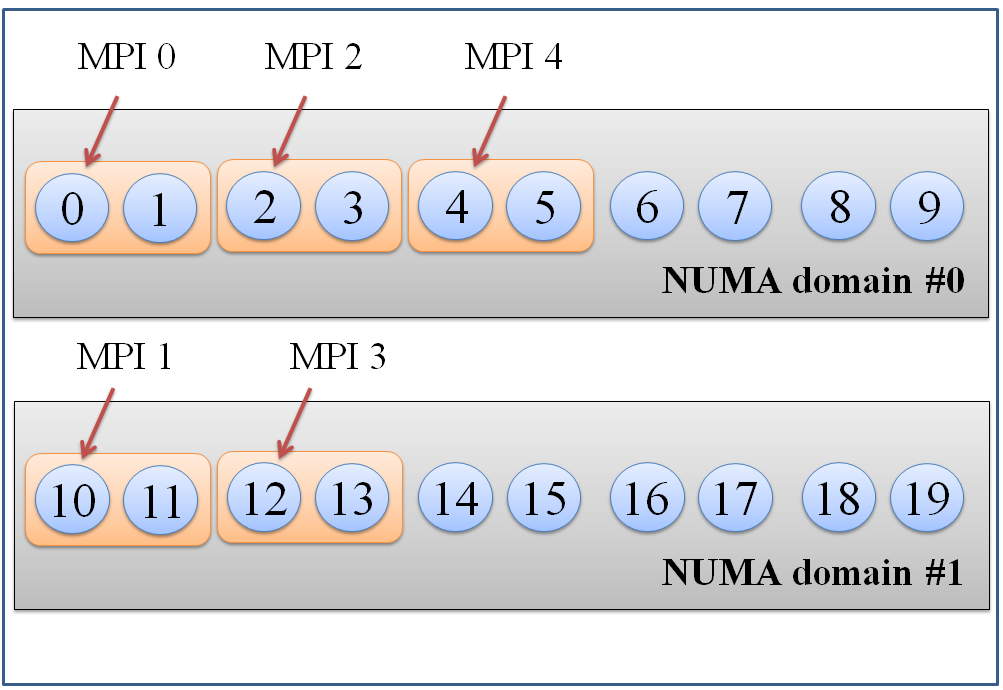
\includegraphics[width=0.45\textwidth]{figures/chapter-2/spread-mode.png}} &
		\subfloat[\textit{Close} mode]{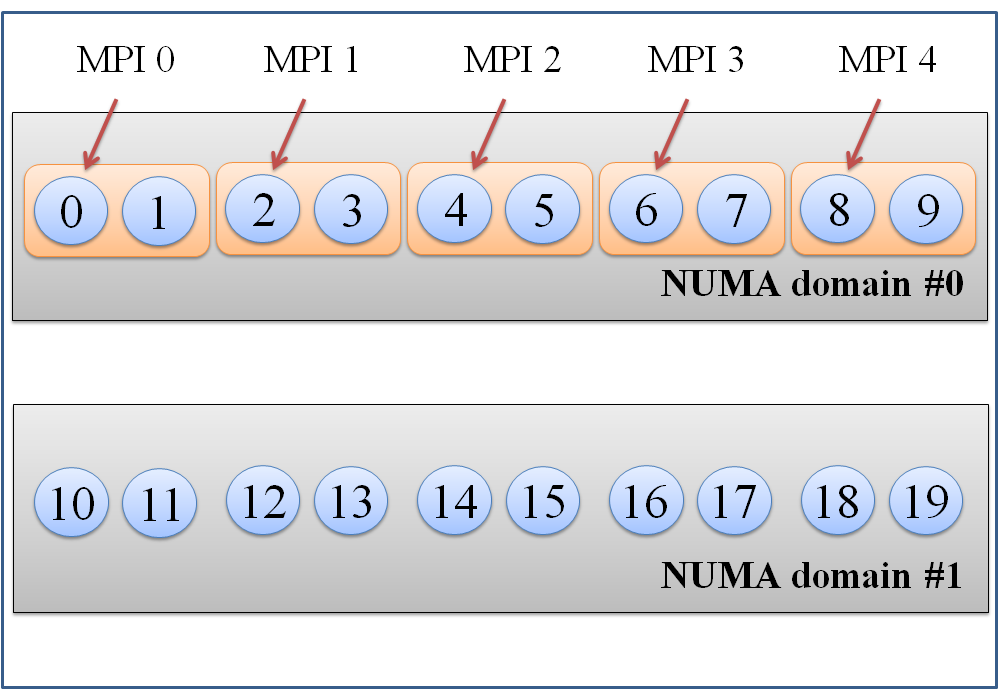
\includegraphics[width=0.45\textwidth]{figures/chapter-2/close-mode.png}} \\
	\end{tabular}
	\caption{An example of process pinning of 5 MPI processes with 2 OpenMP threads per rank in case of HW1}
	\label{fig:python-script-rankfile-example}
\end{figure}



We chose \textbf{Intel 18.2} compiler for this study as the newest and the most efficient Intel compiler at the time of writing.\\
